\documentclass{article}
\usepackage{hyperref}
\hypersetup{
 colorlinks, linkcolor=blue
}
\title{Open-Ended Dynamics of Prediction Games}
\author{Dissertation Proposal\\
    Thomas Willkens
    }
\date{}
\usepackage{algorithm}
\usepackage{algorithmicx}
\usepackage[noend]{algpseudocode}
\usepackage{courier}
\newcommand{\code}{\texttt}
\usepackage{listings}
\usepackage{natbib}
\usepackage{graphicx}
\usepackage[linguistics]{forest}
\usepackage{caption}
\usepackage{subcaption}
\usepackage{amssymb}
\lstset{
  basicstyle=\fontsize{9}{9}\selectfont\ttfamily
}

\begin{document}

\maketitle

\section*{Background}
A core research concern of the artificial life community is the study of
\textit{open-ended evolutionary systems}, which can be broadly defined as evolving systems that
never settle into a single stable equilibrium state. The Earth's biosphere provides the most
obvious example of an open-ended system, as new and ever more complex forms of life have evolved over 
time. However, the emergence of new species through \textit{coevolution} 
provides a challenge for traditional evolutionary models
such as the \textit{replicator equation} which requires the set of species and interactions to be 
fixed and prestated. Rather than model open-ended systems as, for example, a set of diffential equations, 
the recommended approach is to present ``general evolution'' as an algorithmic update equation;
rather than integrating this equation, we must let it evolve and study the \textit{statistics}
of its output (see Chapter 5 in \citep{thurner2018}). 
Open areas of research in the field include the establishment of metrics such as 
\textit{activity} and \textit{complexity} for quantifying open-ended behavior, the 
identification of systems believed capable of open-ended growth, and methods for visualizing 
and interpreting evolutionary dynamics given often massive amounts of data produced in novel 
contexts \citep{packard2019,stepney2021modelling,dolson2020}.

Pioneering work in the field of open-ended evolution includes the identification of punctuated 
equilibria within a variation of the
iterated prisoner's dilemma in \citet{lindgren1994evolutionary}, the self-replicating machine 
code of Tierra and Avida \citep{ray1992evolution,ofria2004avida} and the evolutionary activity 
statistics of \citet{Channon2001PassingTA}. While more recent work such as the Chromaria environment has produced  
systems that exhibit features of open-endedness
by certain metrics \citep{adams2017formal,soros2014identifying}, an unambiguously open-ended 
system has yet to be developed and is considered 
to be one of the ``grand challenges'' of artificial life. The dynamics of these systems in 
general are agreed to be poorly understood, but novel analytical frameworks such as the 
\textit{Measurements of Open-Ended Dynamics in Evolutionary Systems} (MODES) Toolbox have been
proposed to in an effort to better characterize them \citep{dolson2019modes}.

The DEMO Lab of Jordan Pollack has produced much work in the related area of 
\textit{coevolutionary algorithms} (CEAs). CEAs have found practical use on a number of 
difficult problems, such as the sorting networks of \citet{hillis1990co} and the game playing strategies of 
\citet{rosin1995methods}. It has been argued in \citet{togelius2019} that the success 
of some deep reinforcement learning systems such as AlphaStar can be partly attributed to the use of 
competitive coevolutionary principles. However, experimental work by the DEMO Lab showed that 
coevolutionary systems are  prone to unique pathologies that may stall adaptive progress in
certain domains \citep{watson2001coevolutionary}. Theoretical 
work by the lab led to the development of algorithms specifically to address these pathologies
\citep{noble2001pareto, jong2004ideal,de2004incremental}. 

More recently, the lab has begun to explore the potential of coevolutionary dynamics to create
systems capable of open-ended complexity growth \citep{harrington2019escalation,moran2019evolving}. 
This work was cited by Ken Stanley, a leader in the artificial life community, as of special 
interest in a survey paper of the field \citep{stanley2019}. Work by this author \citep{willkens2022} proved that 
previous hypotheses regarding conditions necessary for open-ended growth in these systems,
such as the presence of both cooperative and competitive interactions, in fact do not hold
in the general case. Moreover, certain systems were found to be sensitive to the 
selection method employed, with more sophisticated coevolutionary algorithms producing dramatically
greater rates of complexity growth. It is difficult to picture the behavior of these systems 
from static images and plots alone, and so interested readers are encouraged to view the 
\href{https://docs.google.com/presentation/d/1tklPPoT9hPfJkl9Fy-eHtzVZWNgh4hqUpuVcSHMLBWs/edit?usp=sharing}{presentation slides}
for the 2022 ALIFE conference which include a number of dynamic neural network visualizations.

Work accepted for publication in the 2023 Conference on Artificial Life, ``MODES Analysis of Prediction Games,''
showed that the complexity growth observed in the original work by \citet{moran2019evolving}
cannot be interpreted on face value, and that it may possible
for nonadaptive yet highly complex strutures to emerge through coevolutionary processes. My
work has shown that intuitions often fail us when it comes to understanding the dynamics
of these systems and reveals the need for  a new set of analytical perspectives
when approaching them.

\section*{Chapter 1: Introduction}
The introduction will outline the general aims of the dissertation, summarize the prior 
literature on the subject, and provide an overview of the necessary terminology.

The intent of this work is to pave the way for the understanding and creation of truly open-ended systems 
through a careful statistical analysis of a set of novel yet simple systems known to exhibit forms of
open-ended genotypic complexity growth. We identify
these systems as \textit{coevolutionary prediction games}. They are some of the simplest systems
known to produce such behavior and are therefore ideal for simulation and analysis. The goal is 
to better describe the dynamics of these systems and identify general principles that may apply
to more complex applications such as generative modeling and multi-agent reinforcement learning problems,
as well as features of the natural world.

The substantive contributions of this work include the following:
\begin{enumerate}
    \item The first analytical treatment of prediction games considered as a general class of 
        coevolutionary systems, employing the MODES Toolbox as the primary framework;
    \item The introduction of two new prediction game domains, the \textit{Continuous Prediction Game}
        and the \textit{Harmonic Prediction Game}
    \item The introduction of a new artificial organism model based on the \textit{Genetic Program Parse Tree}
        (GP-Tree) of \citet{Koza92}.
    \item The introduction of a novel visulization and analytical technique, 
        \textit{Qualitative Dynamical Evolutionary Stable State Analysis} (Q-DESSA)
\end{enumerate}

In our experiments, we study the coevolutionary dynamics of populations of 
\textit{artificial organisms} within \textit{coevolutionary ecosystems}.
Organism genotypes are represented as \textit{heterogenous graphs} corresponding to phenotypes
that take the form of \textit{abstract machines}. A coevolutionary system comprises populations
of organisms and interactions that take place between them within a given \textit{interactive domain}.
These interactions often have either a ``cooperative'' or ``competitive'' nature, in which two
organisms will have aligned or opposing interests, respectively.

Each interaction, which is performed in pairwise fashion between all members of two interacting populations, 
yields some measure of \textit{fitness} to each individual involved. Using the results of these 
interactions, a \textit{coevolutionary algorithm} 
produces members of the next generation. A \textit{selection function} chooses which members
have the greatest likelihood to reproduce. For each class of artificial organisms, we define a set 
of \textit{mutation operators} to be stochastically applied to each parent to produce a child
with a modified genotype; in all our experiments reproduction is performed asexually.

We provide here a summary of the artificial organisms under consideration in this dissertation:
\begin{enumerate}
    \item The \textit{Deterministic Finite State Machine} (DFSM) introduced in \citet{moran2019evolving}
    \item The \textit{GNARL Recurrent Neural Network} with operators defined in \citet{willkens2022}
    \item The \textit{Genetic Program Parse Tree} (GP-Tree) based on the Artificial Ant of \citet{Koza92} with 
        modifications novel to this dissertation
\end{enumerate}

We consider four interactive domains:
\begin{enumerate}
    \item The \textit{Linguistic Prediction Game} (LPG) introduced in \citet{moran2019evolving}
    \item The \textit{Collision Game} introduced in \citet{willkens2022}
    \item The \textit{Continuous Prediction Game} novel to this dissertation
    \item The \textit{Harmonic Prediction Game} also novel to this dissertation
\end{enumerate}

We consider two selection functions:
\begin{enumerate}
    \item \textit{Fitness Proportionate Selection} (FPS) where the probability of selection 
        is proportional to the fitness of the organism
    \item \textit{Discovery of Search Objectives} (DISCO), a new selection function based on 
        work by the DEMO Lab specifically to address coevolutionary pathologies \citep{liskowski2016online}
\end{enumerate}

We employ two analytical paradigms:
\begin{enumerate}
    \item The \textit{Measurements of Open-Ended Dynamics in Evolutionary Systems} (MODES) Toobox
        introduced by \citet{dolson2019modes}
    \item The \textit{Q-DESSA} framework novel to this dissertation
\end{enumerate}

\subsection*{CoEvo}
It is necessary to perform these experiments under the same conditions and with the same analytical framework.
For this purpose, the CoEvo framework has developed. Comprising over 8,000 lines of Julia code,
the framework is designed to be modular and extensible and is equipped with an extensive test
suite. Genotypes are stored on disk in stable JLD2 dataformat along with random seeds and other metadata.
It is possible to ``revive'' organisms at any point in the evolutionary timeline to evaluate 
their complexity, study their interactions, and continue their evolutionary progress in a 
reproducible way. 

The framework will be the first of its kind to provide a unified interface for high-performance 
simulation and analysis of arbitrary coevolutionary systems. A link to the repository can be 
found at \href{https://github.com/twillkens/coevo}{here}; it is currently being refactored and
prepared for public release.

\subsection*{Open Science}
The disseration shall be undertaken in the spirit of open science movement 
\citep{vicente2018open}. All code and data
will be made public to members of the scientific community as it is produced. Progress will be 
performed in the open-notebook style, with regular status reports accessible via the Internet.

\section*{Chapter 2: Analytical Methods and Complexity Growth}
Chapter 2 shall outline the statistical methods and analytical approaches to be applied to the
experimental results.

\subsection*{The MODES Toolbox}
The \textit{MODES Toolbox} is a set of metrics and analytical techniques introduced in 
\cite{dolson2019modes} to better understand the open-ended potential of evolutionary systems in terms
 of change, novelty, complexity, and ecology. The toolbox is shown to produce results supporting
  current intuitions and understanding of systems such as rugged NK landscapes and the Avida 
  digital evolution platform \citep{Lenski2003TheEO, KAUFFMAN198711}. 

Before applying the metrics to data resulting from an evolutionary system, it is beneficial to 
first screen out deleterious and neutral genotypes so that the focus is placed on truly adaptive 
mutations. The primary tool for this is the \textit{persistence filter}, 
which has its roots in \textit{coalescence theory}, an area of theoretical population genetics 
\citep{Fu1999CoalescingIT}. This is done by identifying the \textit{persistent lineages} 
according to a sliding window of length $t$ generations. Coalescence theory predicts that in the 
absence of selective pressure, a single individual is expected to become the sole common ancestor 
of the entire population in a median time of $2N$ generations, where $N$ is the population size; 
this value typically becomes much smaller when selective pressure is present. At each generation 
$A - t$, each reproductive individual passes on to its offspring a unique identifier, which is 
passed on their offspring in turn if they are able to reproduce. This continues for $t$ 
generations until $A$ is reached, whereupon the identifiers are collected from members of the 
current population such that the persistent individuals from generation $A - t$ can be 
retrospectively identified.

\begin{figure}[H]
    \begin{center}
        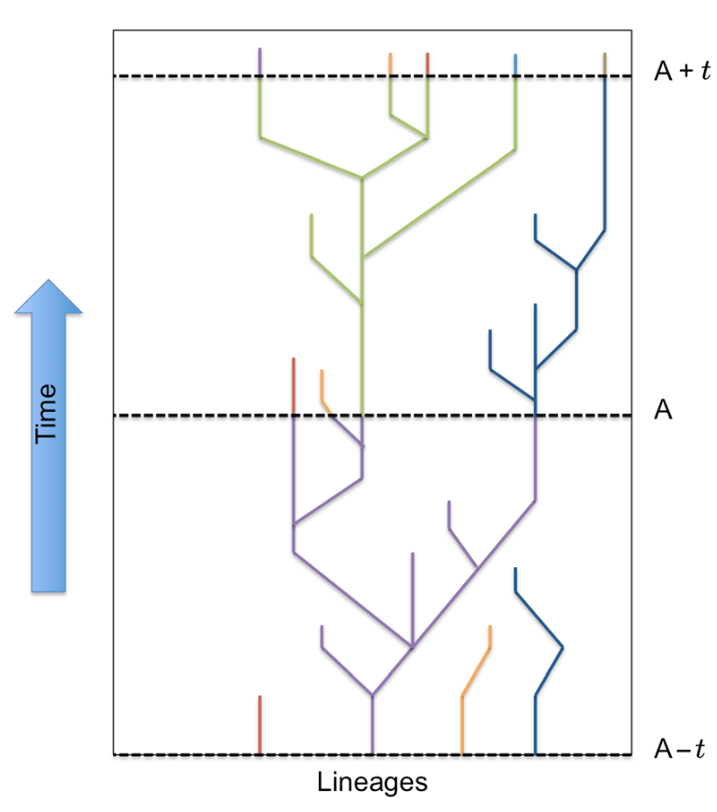
\includegraphics[width=2in]{modes.png}
        \caption{Illustration of persistence filtering taken from \citet{dolson2019modes}.
        At timepoint $A$, the purple lineage has proven to be persistent and therefore the 
        original component from $A - t$ will be considered meaningful. Similarly, the green and 
        blue lineages persist to timepoint $A + t$, and so the original green and blue 
        components will be considered meaningful as they existed at timepoint $A$.}
        \label{modes}
    \end{center}
\end{figure}

This step alone dramatically reduce the volume of data for processing, at least by a factor of 
$N$, but there is more that can be done. It is recommended to identify the 
\textit{informative sites} of these persistent genotypes to prune noncoding genetic material. 
A simple means of doing so is the \textit{knockout} technique: For each site in the genotype, 
remove that site and observe the fitness effect for that individual in its original environment. 
If the fitness either remains the same or increases, this is evidence that the site is nonadaptive 
or not meaningful and can therefore be pruned. There are downsides to this approach as it fails to 
capture interactions between sites. This work will explore the possible use of alternative 
heuristics; preliminary experiments using an incremental fitness-preserving pruning method 
using information relating to the age of the genes have been promising.

Once the persistent individuals and meaningful genotypic sites have been identified, the core 
MODES metrics can be applied at each generation interval $A$ given a window size of $t$:
\begin{enumerate}
    \item \textbf{Change}: A count of the number of unique persistent genotypes at generation 
        $A$ that are different than those at generation $A - t$;
    \item \textbf{Novelty}: A count of the number of persistent genotypes in generation $A$ 
        that have not been seen at all in the intervals preceding it;
    \item \textbf{Complexity}: The greatest count of informative sites among all persistent 
        genotypes at generation $A$;
    \item \textbf{Ecology}: The Shannon entropy obtained from measuring the proportion of the 
        persistent population occupied by each unique genotype at generation $A$. This metric 
        provides an intuitive notion of diversity or evenness, as its value grows higher as a 
        greater number of unique genotypes occupy more equal proportions of the population. 
\end{enumerate}

\subsection*{Q-DESSA}
The MODES toolbox provides an excellent set of analytical tools for explicating core dynamics of 
evolutionary systems. However, while we get an overall sense of the growth and behavior of the
system, we do not gain a sense of how two systems that exhibit similar MODES dynamics might differ.
For example, two systems might both exhibit cycling behavior, evidenced by a negative slope of
the novelty metric. But we do not get a sense of the frequency of the cycles, the geometry of
the genotype space, or the regions in which those cycles occur.

The visualization framework presented in \cite{dolson2020}, in particular the \textit{lineage trajectories} 
drawn over a fitness landscape, provides inspiration for how to approach this problem. The 
problem is that in our coevolutionary setting, the fitness function is not fixed and we have
multiple populations of interacting individuals.

\textit{Q-DESSA} (Qualitative Dynamical Evolutionary Stable State Analysis) is a proposed method for 
analyzing these aspects of potentially open-ended systems. The method employs a graph neural
network component trained in an unsupervised fashion over the dataset of persistent organisms 
filtered using MODES. An advantage of all the models considered in our prediction game is that 
they have a natural graph representation, and so this method can be applied 
in similar fashion to each. We collect together the set of all persistent individuals across all trials of all
ecosystems for a given artifical organism type. An approach such as the \textit{UGraphEmb framework}
\citep{Ding2019UNSUPERVISEDIW} may be employed to obtain graph-level embeddings that
reflect the \textit{graph edit distance} between the genotypes of the organisms. In such a fashion we can
derive a vector space in which the embeddings of the two graphs preserve their graph-graph 
proximity.

In \cite{Ding2019UNSUPERVISEDIW}, the resulting embeddings are reduced in dimensionality using 
\textit{t-distributed Stochastic Neighbor Embedding} (t-SNE) and visualized in a 
2D space \citep{van2008visualizing}. However, it is known that t-SNE may prioritize local structure
at the expense of global structure, which can introduce significant distortion resulting in 
misleading interpretations; to mitigate this, we plan to experiment with the recent PaCMAP
dimensionality reduction method which is believed to produce a better tradeoff between local and
global structure \citep{wang2021}. The UGraphEmb framework uses the \textit{graph edit distance}
as a measure of similarity between graphs, which we plan to implement using the GEDLIB C++
framework \citep{Blumenthal2019GEDLIBAC}. Experiments are currently being performed using the 
difference between the Laplacian spectra of the graphs as a measure of similarity as in 
\cite{deLang2014}, which is fast to compute but provides less precision as edge and node label
information is lost.

\begin{figure}[H]
    \begin{center}
        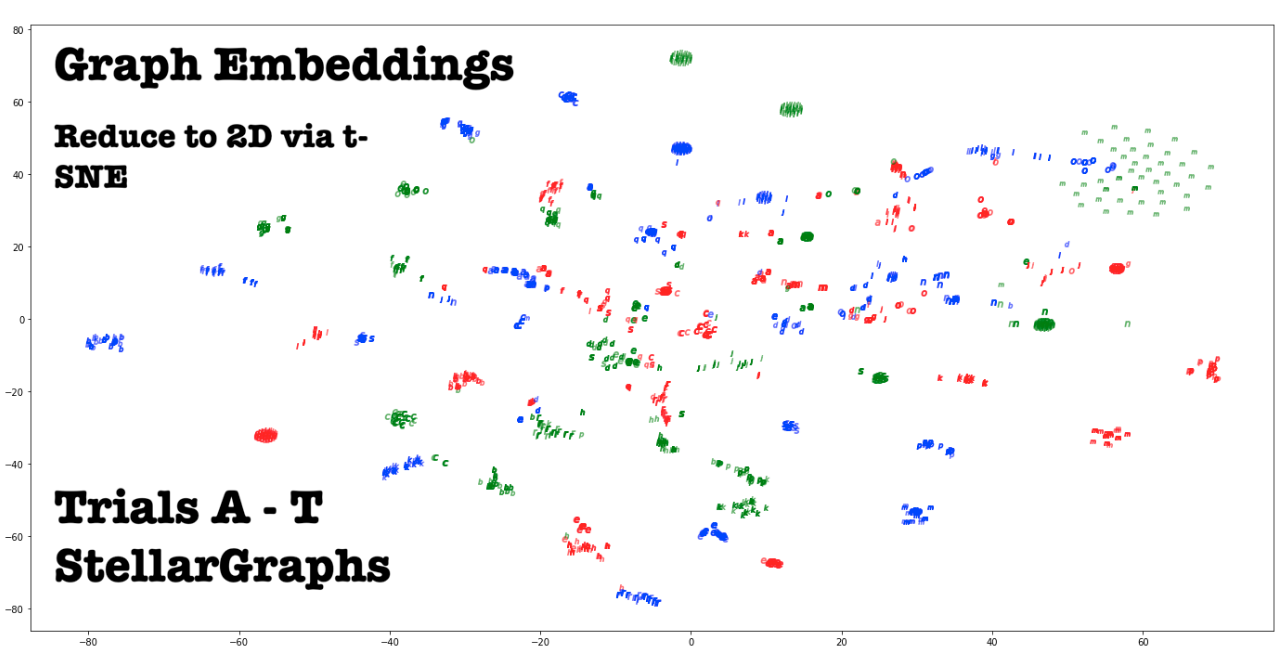
\includegraphics[width=3.5in]{embeddings-stellar.png}
        \caption{This figure from preliminary experiments represents the reduced embeddings of GNARL neural networks, where 
        the colors denote the species of each organism and the letters A-T represent the trial number 1-20.
        This was produced using the StellarGraph Python library from experimental data taken from the final generation.
        Despite some distortion and error, the resulting embeddings capture the intuitive notion 
        that members of one population tend to be clustered together in the embedding space. The 
        full Q-DESSA approach would produce lineage trajectories for organisms that pass the MODES filter.}
        \label{dfsm}
    \end{center}
\end{figure}

As an analogy, we may borrow concepts from the dynamical systems theory of \citet{strogatz:2000}, considering each 2D reduced
embedding as a \textit{phase point} in a dynamical system. In this sense, each point taken from a lineage 
at generation
$A$, $A + t\dots$ forms a \textit{trajectory} in the phase space. The path the trajectory takes 
reflects the evolutionary dynamics of the system, and by considering the trajectories taken
by different species within each ecosystem, we can better understand the evolutionary relationship
between each population. It may be possible then to qualitatively identify the presence of evolutionary stable
states as well as to classify them according to the terminology of \citet{watson2001coevolutionary}:

\begin{enumerate}
    \item \textit{Disengagement}: When the trajectories of two or more population do not leave some 
        \textit{fixed-point region} of the space. As these systems are out of equilibrium, and
        there always exists the mutational possibility of components being added or removed from
        the genome and we do not expect a true fixed point to emerge. But orbits constrained within
        a region reflect that the populations have disengaged evolutionarily and that no more 
        complex adaptations are expected to occur.
    \item \textit{Convention chasing}: When the trajectories of two or more populations orbit between two
        or more \textit{semi-stable regions}. This is a situation where populations cycle through a limited 
        number of adaptive solutions and better solutions either do not exist or are
        not reachable through mutation. 
    \item \textit{Open-ended behavior}: When the transient phase of the trajectory continues indefinitely,
        and there are no fixed points or semi-stable regions. Open-ended growth necessarily implies
        open-ended behavior, as a lineage with genotypes that tend to grow over time without 
        bound will not remain within any region.
\end{enumerate}

\begin{figure}[H]
    \begin{center}
        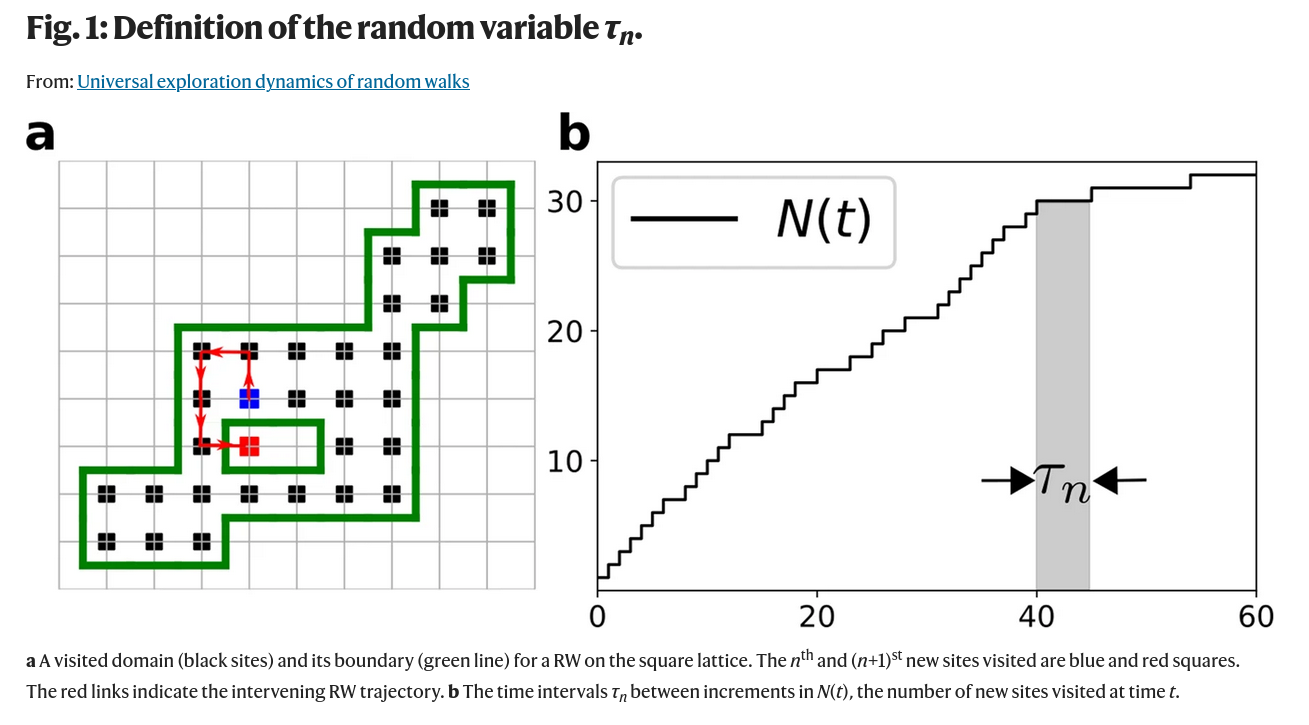
\includegraphics[width=4.5in]{random-walker.png}
        \caption{Site visitations and waiting time plot, taken from \cite{Regnier2023}}
        \label{walker}
    \end{center}
\end{figure}

To quantify these notions in a stastical fashion, we propose that the theory of random walks 
could be applied as in \cite{Regnier2023}. By dividing the embedding space into a lattice, we can examine metrics 
such as the number of distinct sites visited by a lineage, as well as the waiting time $\tau_{n}$,
which is the time taken to reach a new, distinct site. This will only approximate the true dynamics
of the underlying system given the inevitable distortion of dimensionality reduction and training
error, but it could provide more insight than the MODES metrics in isolation.

\section*{Chapter 3: The Linguistic Prediction Game and the Complexity of DFSMs}

This chapter will finish work begun in \citet{moran2019evolving} and continued in a paper 
accepted for publication in the 2023 Conference on Artificial Life titled 
``MODES Analysis of Prediction Games.'' 

The \textit{linguistic prediction game} is a simple two-player coevolutionary domain. 
For an infinite sequence of timesteps, each player simultaneously emits a bit. If the game is \textit{cooperative}, then players share 
the same goal: either to match (or mismatch) the bit provided by the other. 
In a \textit{competitive} interaction, however, only one player is rewarded for matching 
(or mismatching) bits. Neither player is aware of the nature of their relationship upon starting
the game, and their decisions must be made based solely on the patterns of bits produced.
 
Organisms in the game take the form of \textit{deterministic finite state machines} (DFSMs). 
Each state has either a 0 or 1 label, corresponding to the bit emitted at that state, and two 
transition links. The bit emitted by the other player determines which of the links to choose to 
transition to the next state. Due to the discrete nature of the machines, a loop eventually must 
occur. The simulation ends once such a loop is detected, and the score for each player is 
determined by taking the average of all their scores in the loop.

\begin{figure}[H]
    \begin{center}
        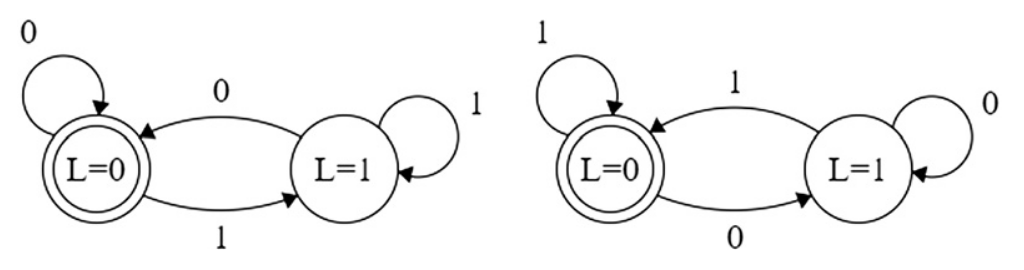
\includegraphics[width=4.5in]{dfsm.png}
        \caption{Two examples of DFSM organisms. Node labels indicate the symbol to be emitted 
        at that state, while transition labels indicate the symbol emitted by the other 
        that causes the transition to occur.}
        \label{dfsm}
    \end{center}
\end{figure}

Evolution begins with identical populations consisting of a single \textit{start state} with two 
links to itself. There is an equal probability that one of 
four mutations will occur: (1) Add state, (2) remove state, (3) flip state label, (4) reassign link.

\begin{figure}[H]
    \begin{center}
        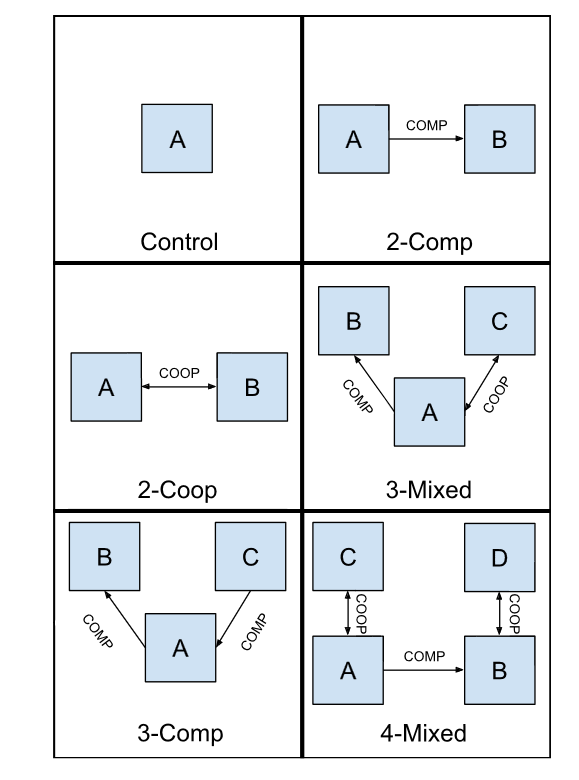
\includegraphics[width=3.5in]{ecosystems.png}
        \caption{Figure taken from \cite{moran2019evolving}}
        \label{ecosystems}
    \end{center}
\end{figure}

The primary ecosystems to be studied include the following:
\begin{enumerate}
    \item In the \textit{Control} ecosystem, populations evolve without the presence of selective pressure.
        The results are used to interpret the open-ended behavior of the other ecosystems.
        In general, genetic drift will lead the size of the organisms will increase gradually 
        over time due to the fact that the number of states is bounded at one.
    \item The \textit{Two-Species Competitive} (Comp) ecosystem involves two populations: one 
        whose members seek to match bits, and another whose members seek to mismatch.
    \item In the \textit{Two-Species Cooperative} (Coop) variety, both seek either to match or 
        to mismatch. 
    \item In the \textit{Three-Species Mixed} (3-Mixed) variety, one ``host'' species is in a 
        cooperative relationship with one population and a competitive relationship with a ``parasitic'' other. 
    \item In the \textit{Three-Species Competitive} (3-Comp) variety, all three species are in competition.
    \item In the \textit{Four-Species Mixed} (4-Mixed) two cooperating pairs of species are linked by 
        a single competitive relationship.
\end{enumerate}

It was argued that ecosystems possessing only cooperative or competitive interactions tend to 
plateau in terms of complexity, there defined as the count of the number of states once a DFSM 
is pruned using \textit{Hopcroft's algorithm} \citep{Hopcroft1971AnNL}. Meanwhile, 
\textit{mixed} ecosystems were believed to hold the potential for \textit{unbounded growth}, 
there determined as when the slope of the line of best fit to the mean complexity growth of a 
population exceeds that of a control or ``shadow'' ecosystem that lacks selection pressure. 

A number of hypotheses were proposed to explain the behavior of the systems. These include that 
primarily cooperative species are more likely to exhibit growth; that \textit{convention chasing} 
may be responsible for cycles between competitive species, leading to 
\textit{evolutionary stable states}; and that clusters of competitive interactions appear to 
choke growth in larger configurations, leading to \textit{degenerate ecosystems} 
\citep{Ficici1998ChallengesIC,watson2001coevolutionary}. However, more comprehensive theoretical and statistical 
justification was left for future work, as the volume and apparent intricacy of the machines 
and their interactions made manual inspection and analysis intractable over evolutionary timescales. 

\begin{figure}[H]
    \begin{center}
        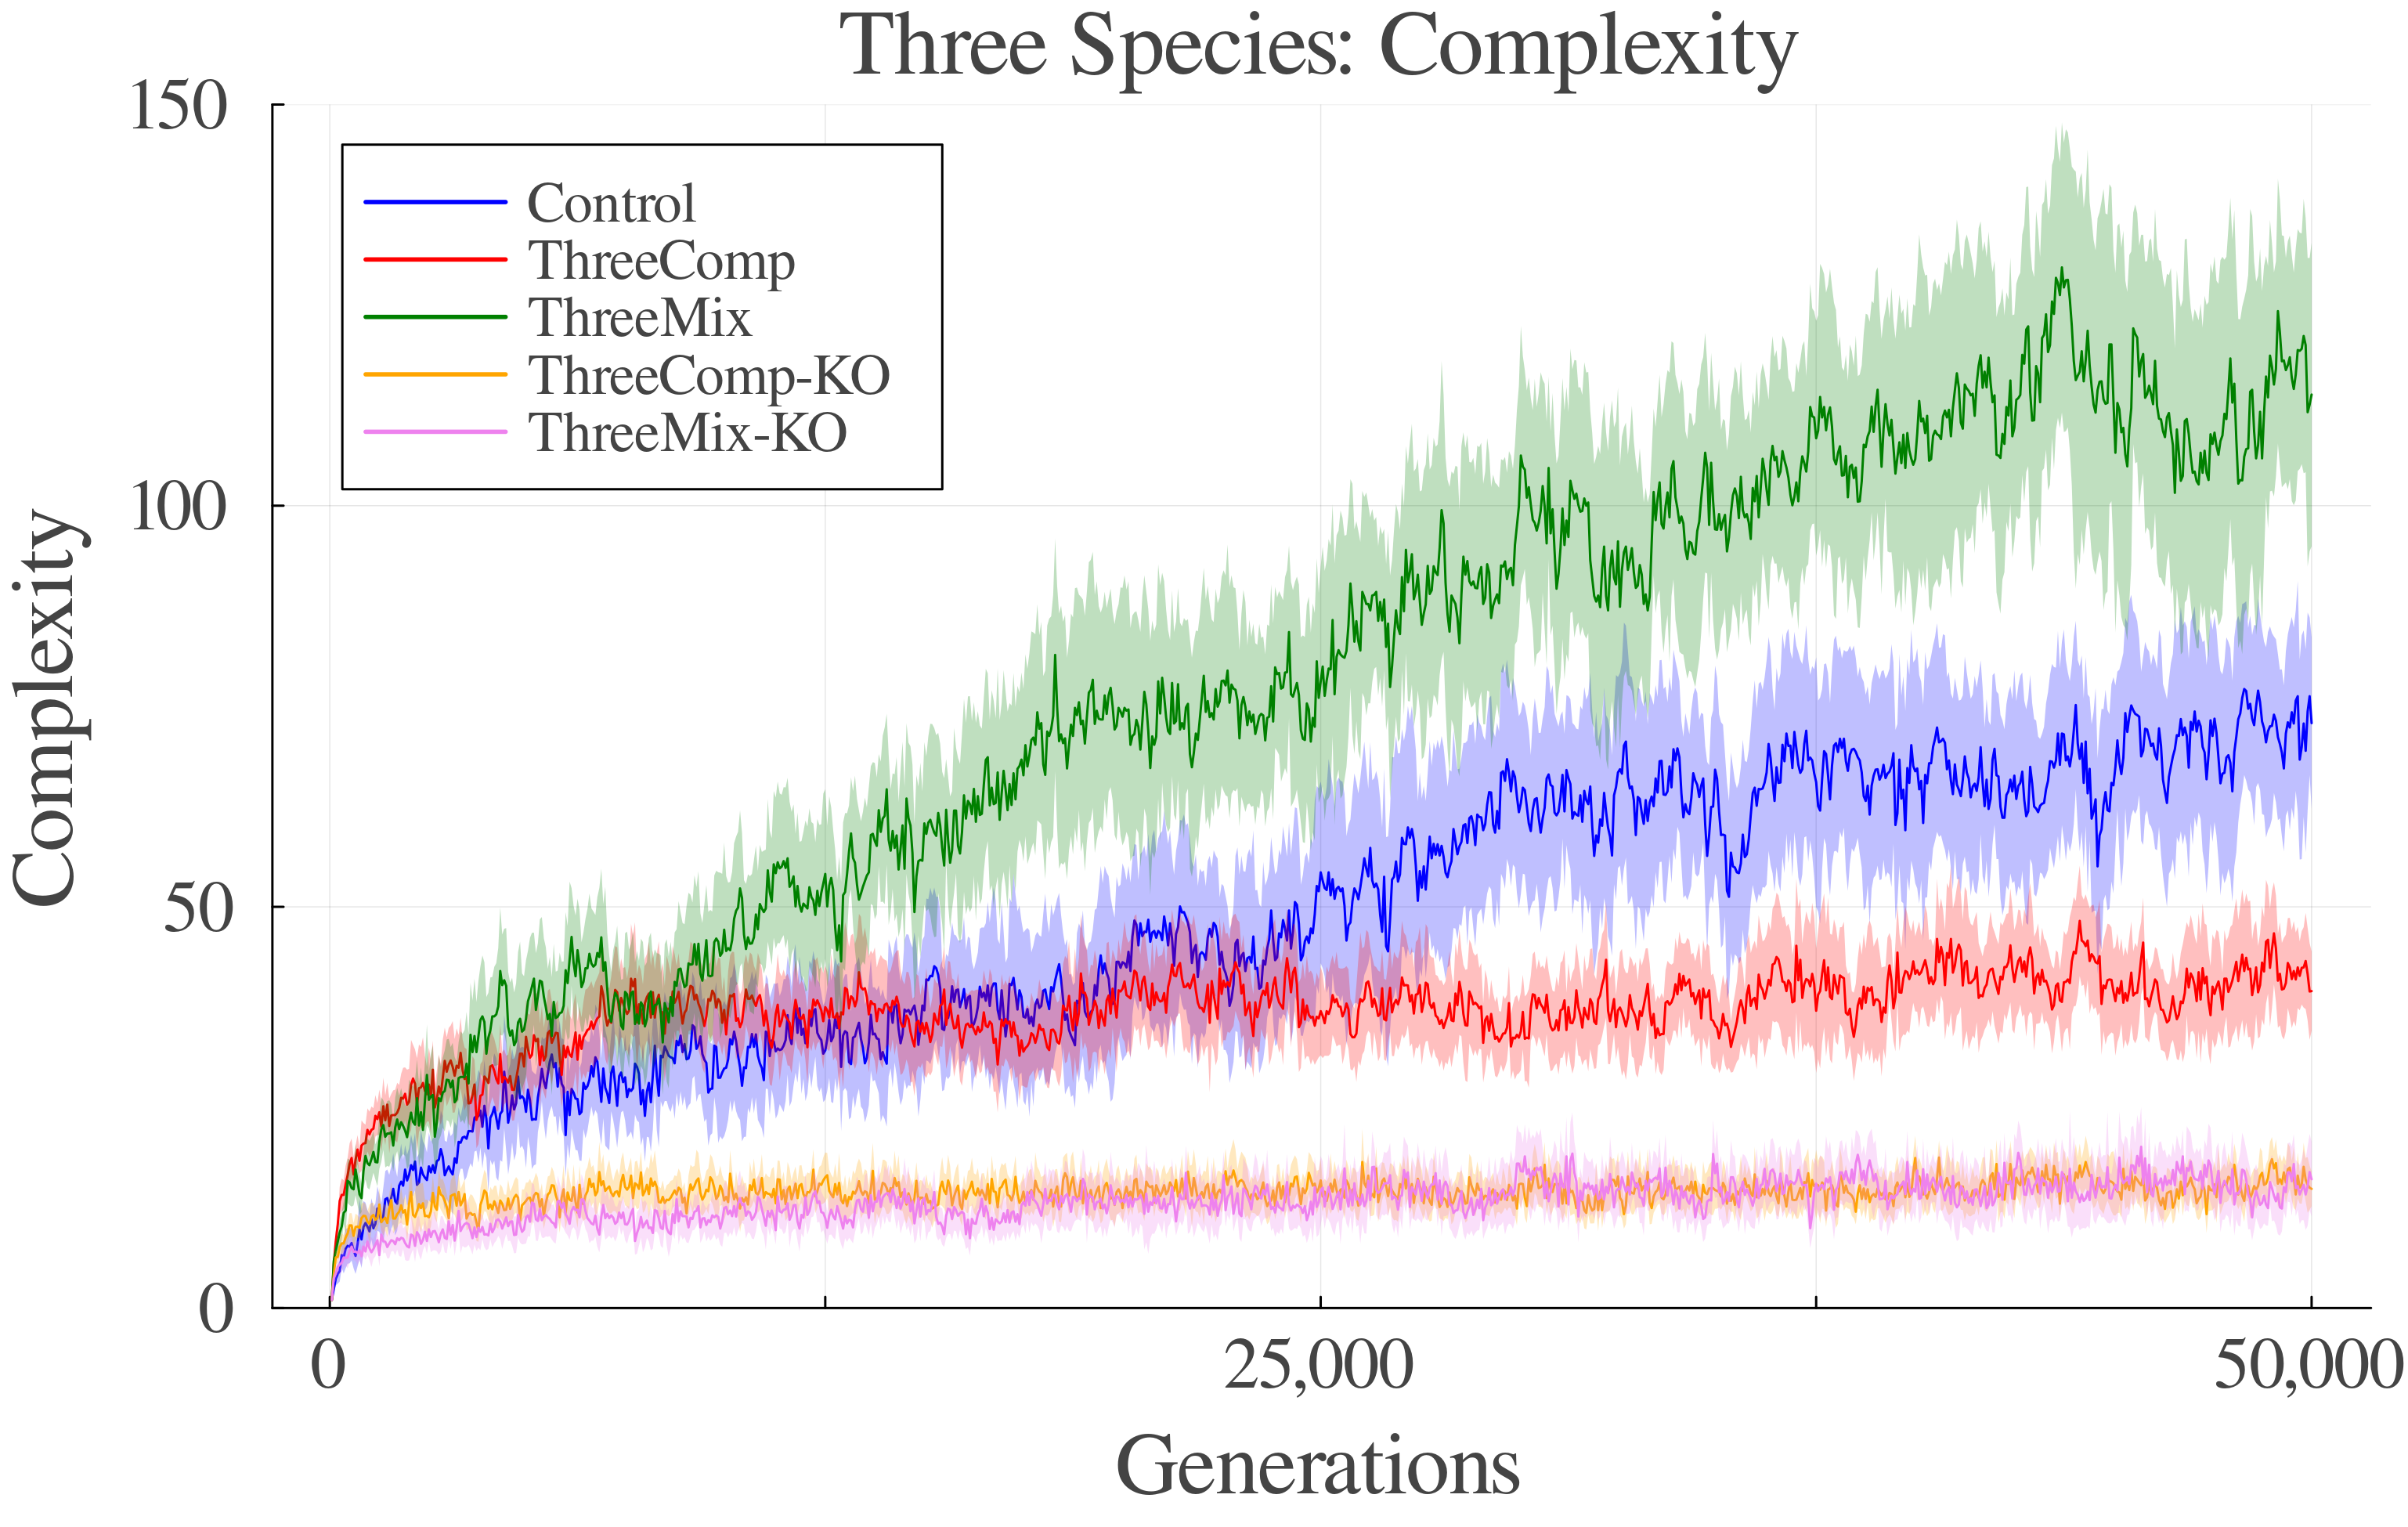
\includegraphics[width=3.5in]{3complex.png}
        \caption{Figure taken from the upcoming publication ``MODES Analysis of Prediction Games''
        The complexity growth of the \textit{adaptive knockout} group (3-Mixed-KO, pink line), is well below that 
        of the Hopcroft group (3-Mixed, green line). This suggests that the observed growth is 
        largely nonadaptive, but the mechanisms behind this behavior are not yet understood and will 
        be a subject of investigation.}
        \label{ecosystems}
    \end{center}
\end{figure}

\subsection*{Goals}
This chapter will employ MODES Toolbox, the Q-DESSA method, and the DISCO selection method to
answer the following open scientific questions:
\begin{enumerate}
    \item Is the complexity growth observed in mixed ecosystems adaptive or nonadaptive upon 
        application of the MODES metrics? Preliminary evidence suggests that a large portion of 
        the growth is nonadaptive.
    \item Can competitive ecosytems be statistically shown to demonstrate convention-chasing 
        or cycling behavior?
    \item Preliminary experiments suggest that the original work by \citet{moran2019evolving}
        failed to adequately characterize the behavior of various ecosystems given different
        ``competitive'' and ``cooperative'' configurations. Can the 
        underlying dynamics be better characterized and understood?
\end{enumerate}

\section*{Chapter 4: The Collision Game and the Growth of GNARL Networks}
\subsection*{The Collision Game}
See the \href{https://docs.google.com/presentation/d/1tklPPoT9hPfJkl9Fy-eHtzVZWNgh4hqUpuVcSHMLBWs/edit?usp=sharing}{presentation slides}
for the 2022 ALIFE conference which include a number of dynamic visualizations.

The \textit{collision game} is a parameterized finite-horizon two-player game introduced in 
\citet{willkens2022} that takes place on a real-valued one-dimensional number line. On 
timestep zero, each agent is assigned a position on the line such that they are some distance 
apart. At every timestep, each agent emits two real-valued outputs between -1.0 and 1.0.
The first is a \textit{movement} value, which is summed with the agent's current position value 
to determine its position at the next timestep, while the second is a \textit{communication} value. 

At the start of the next timestep, each player is provided with the distance between their two 
respective positions along with the communication value of the other agent. Each then determines 
new action and communication values, and so on. The episode ends upon one of two conditions: If 
the position of the agent that began with the lesser value becomes greater than or equal to the 
position of the other, the game is over and the interaction is classified as a \textit{collision}; 
however, if the agents fail to collide by some specified timestep, it is an \textit{evasion}. 

The linguistic prediction game and the collision game differ in various ways: 
The former is infinite-horizon, with discrete actions and a one-dimensional action space; 
meanwhile, the latter has finite-horizon episodes, real-valued actions, and a two-dimensional 
action space. Moreover, the collision game features three classes of interaction:
\begin{itemize}
    \item \textit{Affinitive}: If the episode terminates with a collision, both agents are rewarded with a single point; otherwise neither agent is rewarded. We classify this as a \textit{cooperative} relationship as both interests are aligned.
    \item \textit{Avoidant}: Both agents are rewarded if no collision occurs and are given nothing otherwise. This also is a \textit{cooperative} relationship, but one incentivizing a different pattern of behavior.
    \item \textit{Adversarial}: One species is assigned the role of predator, the other the prey. If the episode ends with a collision, the predator is awarded a point while the prey receives nothing, and vice-versa. This is a \textit{competitive} relationship due to the misalignment of their goals.
\end{itemize}
We note that the reward in the linguistic prediction game is real-valued, while in the collision 
game it is discrete. But there are strong similarities between the two games:
They can be easily mapped to various ecosystem topologies, 
agents begin with ignorance of their partner's identity, different flavors of competitive 
and cooperative interactions are involved, and there is room for diverse strategies to emerge.

\begin{table}[t]
    \begin{center}
\begin{tabular}{ c|c|c } 

  & \textit{Collision} & \textit{Evasion} \\ 
 \hline
 Affinitive & (1, 1) & (0, 0) \\ 
 Avoidant & (0, 0) & (1, 1) \\ 
 Adversarial & (1, 0) & (0, 1) \\ 
 \hline
\end{tabular}
        \caption{Payoffs for the collision game}
        \label{fig:payoffs}
    \end{center}
\end{table}

\subsection*{GNARL Networks}
The abstact machine chosen to represent the organism model in this experiment is the recurrent GNARL
network as described in \cite{angeline1994}. GNARL networks evolve both their weights and 
topologies starting from a minimal state. Our networks here have two input nodes corresponding 
to the distance and communication value of the other agent, one bias node, and two output nodes 
corresponding to the movement and communication actions. The first generation has zero hidden 
nodes and zero connections.

Each node output is the weighted sum of all incoming connections passed through a nonlinear 
function. We use the \textit{tanh} activation function for all connections so that output is 
bound in the range $[-1.0, 1.0]$. Each node retains this output value as a hidden state; in the 
case of a self-loop, the state value from the prior activation is weighted and likewise included 
in the sum. The movement action of the \textit{greater} (or rightmost) agent is negated in simulation, 
so that an output of 1.0 always corresponds with moving towards the other agent and -1.0 with retreat. 

\begin{figure}[H]
    \begin{center}
        %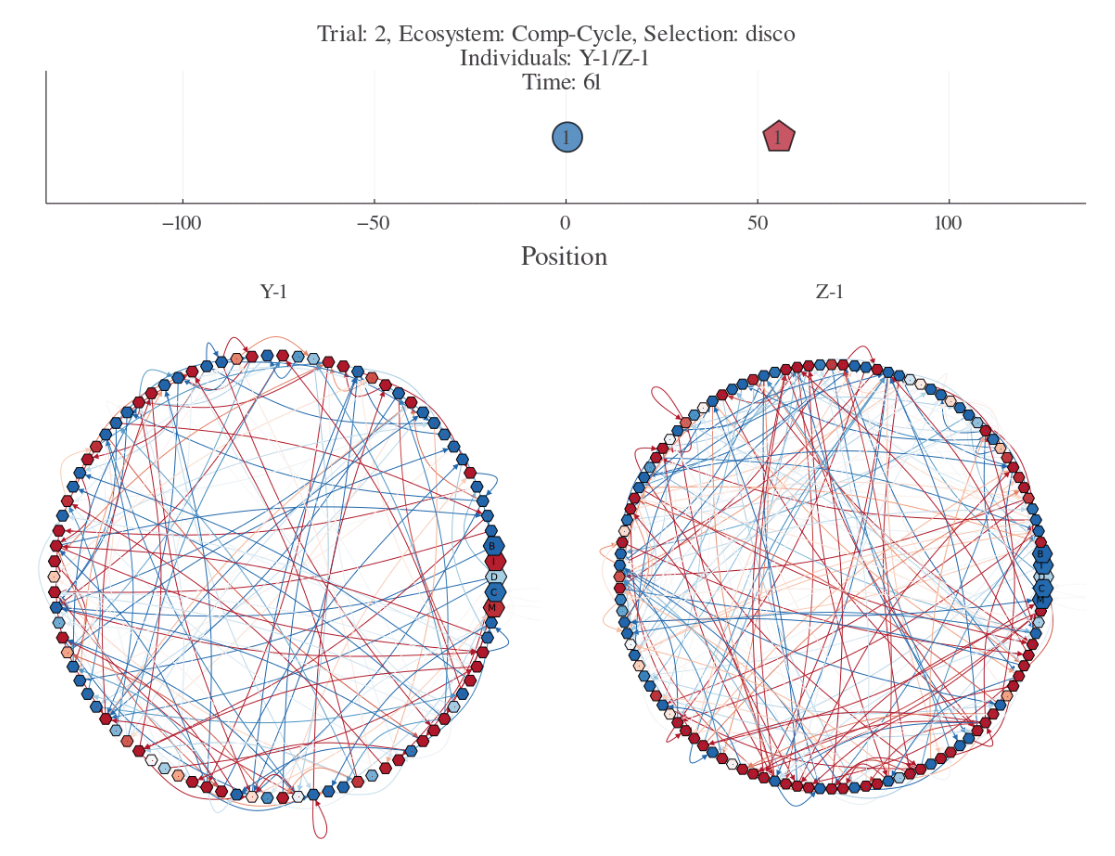
\includegraphics[width=2.1in]{gnarl.png}
        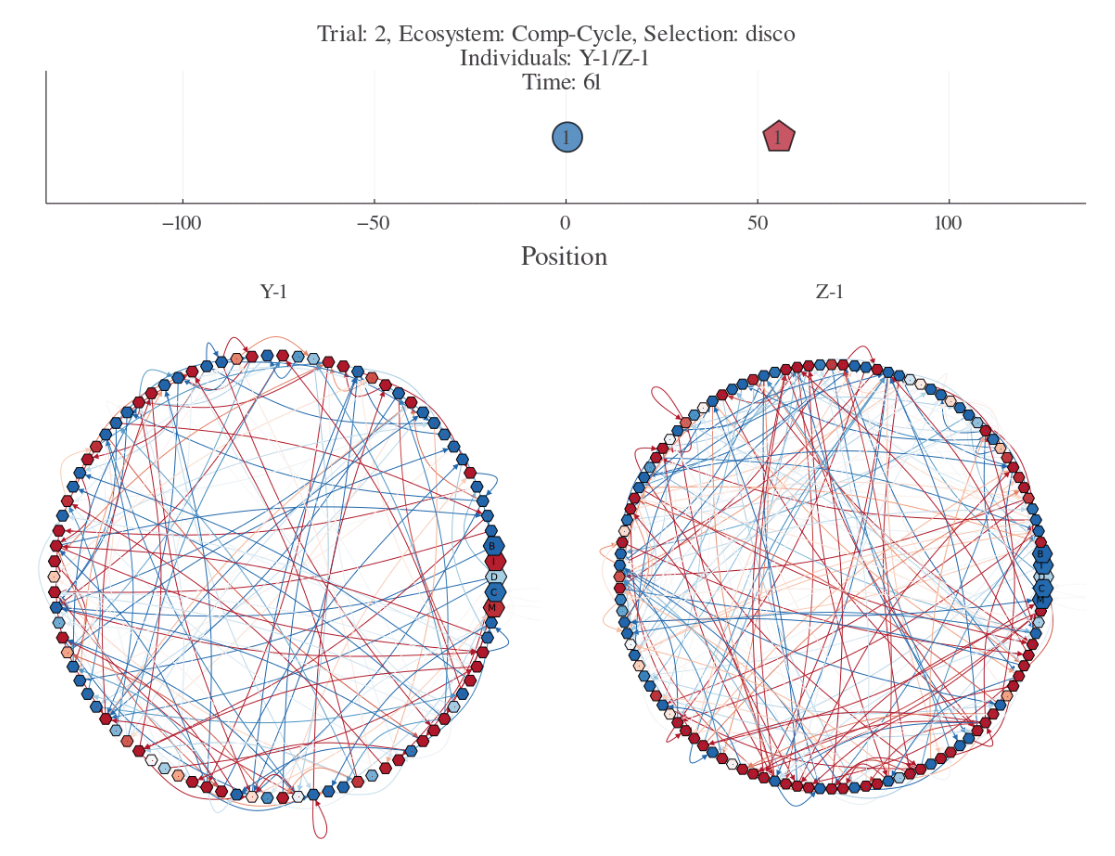
\includegraphics[width=4in]{gnarl.png}
        \caption{Complex GNARL Networks at one timestep of an interaction in the collision game
        \citep{willkens2022}. The state of each node and its weighted outputs is represented by 
        color, with red being values close to -1.0 and blue being values close to 1.0.}
        \label{gnarl}
    \end{center}
\end{figure}

\subsection*{Goals}
In \citet{willkens2022}, it was found that rates of complexity growth followed different 
patterns than those predicted by \citet{moran2019evolving}. Moreover, for all the ecosystem
configurations considered, fitness-proportionate selection failed to produced unbounded
complexity growth, while the DISCO selection method succeded in some. This chapter will investigate the
following questions using the MODES Toolbox and the Q-DESSA method:
\begin{enumerate}
    \item How does the DISCO selection method affect evolutionary dynamics such that 
        unbounded complexity growth is produced in the collision game?
    \item Is the complexity growth adaptive or nonadaptive by the standards of the MODES Toolbox?
    \item Will open-ended transients be observed upon application of the Q-DESSA method?
\end{enumerate}

\section*{Chapter 5: The Continuous and Harmonic Prediction Games with Genetic Programming}
Here we introduce two new domains predicted to exhibit open-ended characteristics. 

The first, the \textit{continuous prediction game}, may be considered a variant of the linguistic
prediction game. The game can be envisioned as a pursuit about the unit circle. Each agent has a
position corresponding to a point on the unit circle, beginning at the same point. At each timestep,
each agent is given a scalar observation corresponding to the arclength distance between the two agents
Each agent then produces a scalar action value, which is applied to produce a rotation of that point
on the unit circle. The distance between the two points is measured and subjected to a scoring function 
and the process repeats for a given number of timesteps. The overall score is the average over 
all timestep scores in the episode and is illustrated in Figure \ref{continuous}.

In this game, a ``cooperative'' interaction is defined as one in which each agent is rewarded for minimizing the
distance between the two points on each timestep, while in a ``competitive'' interaction, one
will seek to minimize the distance while the other is rewarded for maximizing it. 

The second, the \textit{harmonic prediction game}, springs from the observation that the 
``distance'' function in such prediction games is ultimately arbitrary, and that multidimensional
outputs and inputs may be interpereted in creative ways. If a domain provides sufficient 
adaptive pressure and coevolutionary tension, we could expect to observe various forms
of open-ended complexity across a wider range of representations.

\begin{figure}[H]
    \begin{center}
        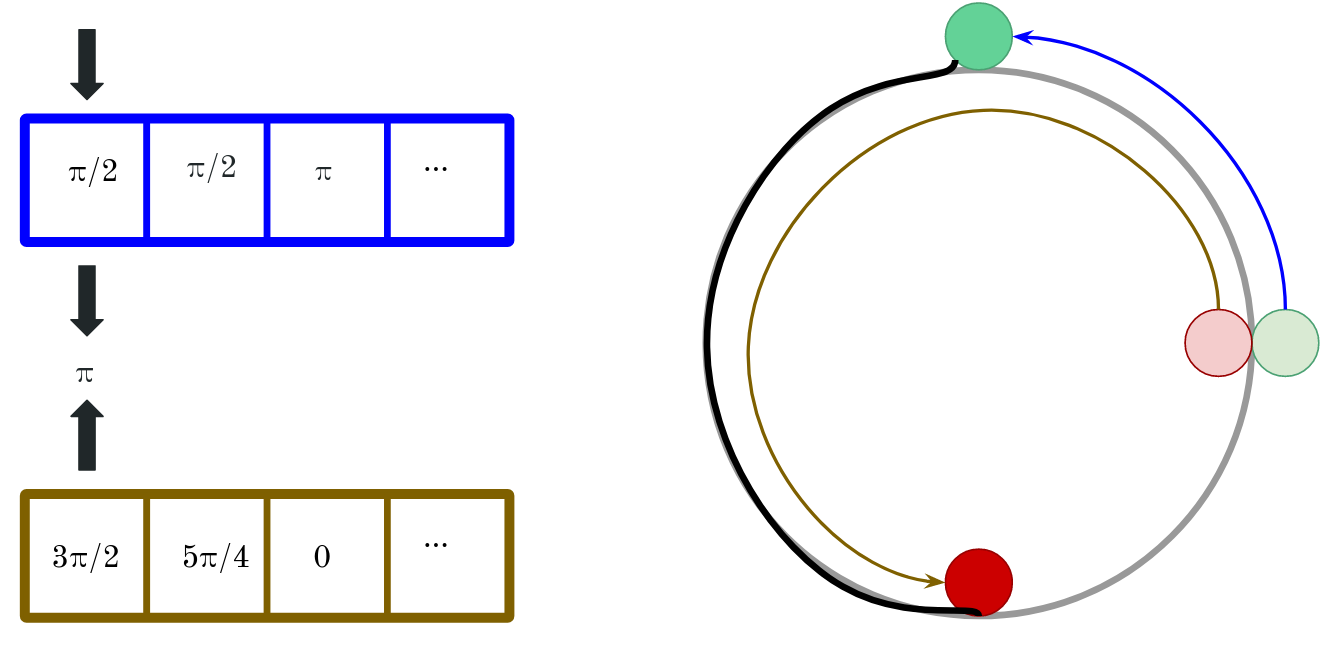
\includegraphics[width=4.5in]{con2.png}
        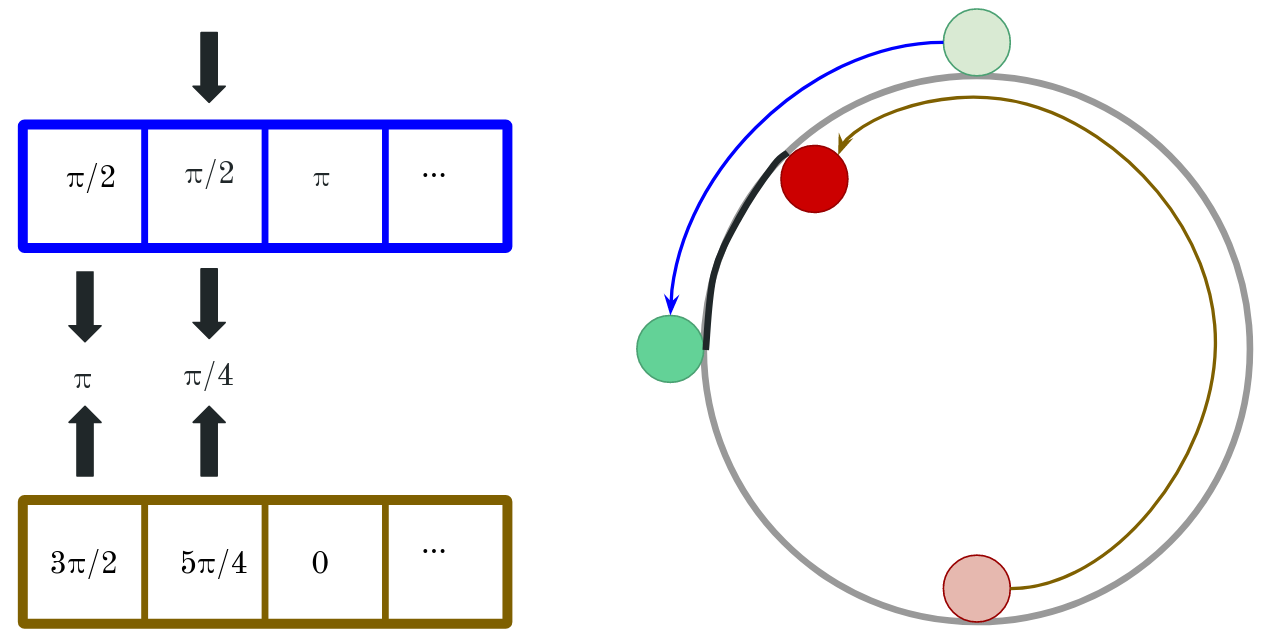
\includegraphics[width=4.5in]{con3.png}
        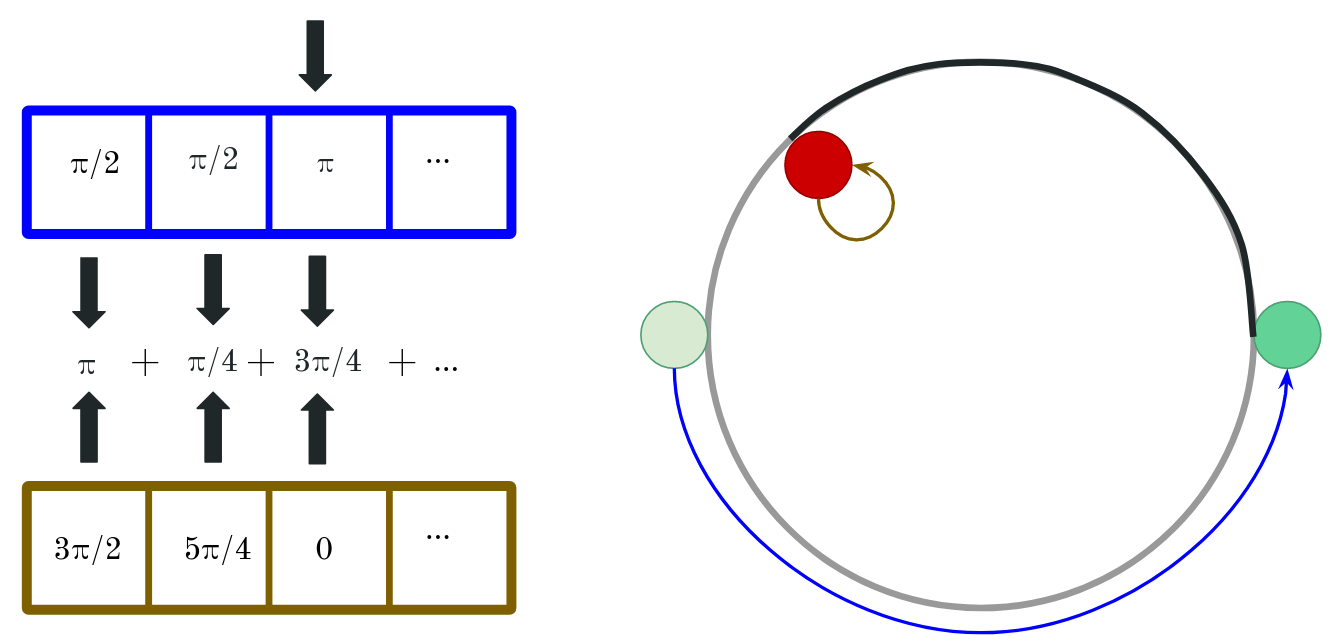
\includegraphics[width=4.5in]{con4.png}
        \caption{Example of scoring in the continuous prediction game.}
        \label{continuous}
    \end{center}
\end{figure}


The harmonic prediction game interprets each scalar observation as the frequency of a 
synthesized tone. As an alternative ``distance'' metric, we may use a \textit{dissonance model}
such as that of \citet{sethares2005}
as presented in \citet{cook2017} and shown in Figure \ref{cook}. The interval created by the harmony of the two tones 
may be then measured using the dissonance model; a ``cooperative''
interaction is one in which both are rewarded for producing harmony, 
while a ``competitive'' interaction corresponds
to when one agent is rewarded for producing harmony, while the other is 
rewarded for producing dissonance. The resulting score is not expected to reflect human aesthetic
prefences, but we predict the emergence of patterns that are neither trivial nor random.

\begin{figure}[H]
    \begin{center}
        %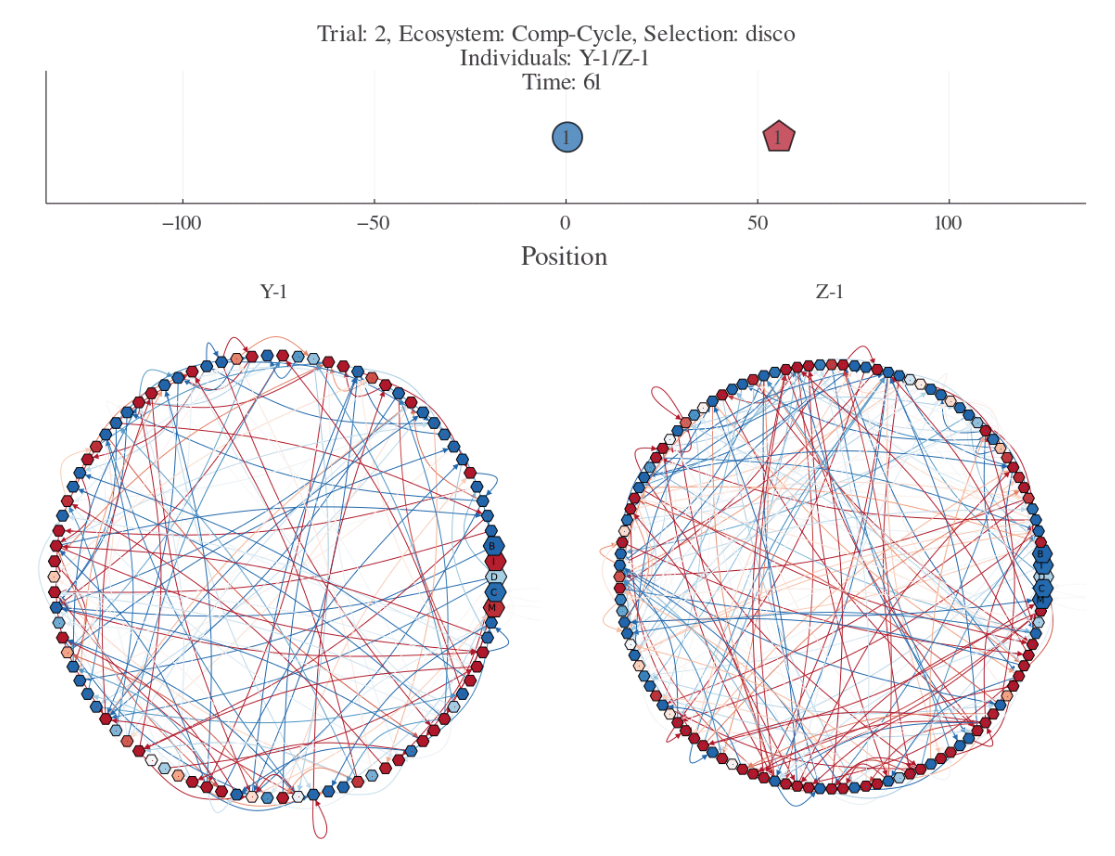
\includegraphics[width=2.1in]{gnarl.png}
        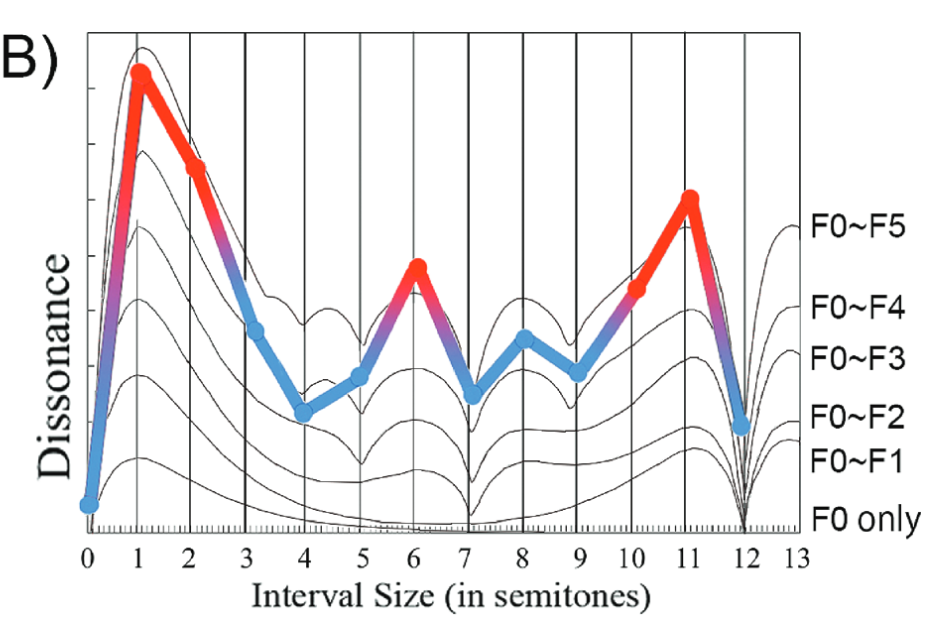
\includegraphics[width=4.5in]{cook.png}
        \caption{Dissonance model shown in \citet{cook2017}. The colored line represents the 
        empirical curve of perceived dissonance reported by human subjects, while the black 
        lines represents the addition of 
        overtones to the theoretical model of \citet{sethares2005}.}
        \label{cook}
    \end{center}
\end{figure}

\subsection*{Genetic Programming}
As a third substrate, we will use constructs from the \textit{genetic programming}
paradigm to represent our artificial organisms. We use the Artificial Ant automata 
along with the Symbolic Regression framework as presented 
in \citet{koza2005} as a basis. The difference is that in addition to protected arithmetic operations,
we also include operations for writing values to an output tape and reading values produced by
the other agent from its own respective output tape. These tapes will begin with a single entry
of real value and grow in length over the course of the episode.

Different representations are currently under investigation. The tapes may be read in a circular
fashion, where each read operation moves the read head forward one position, and reaching the
end returns the tape to the beginning; see Figure \ref{fig:gp2} for one simple example. Alternatively, we 
could employ a noncircular tape with terminals for moving the read head backwards and forwards. 
Additional computational power could be provided by equipping each organism with a stack, 
along with operations for pushing and popping values resulting from intermediate calculations.

The tradition depth-based GP mutation operator can be highly destructive and is stochastic in the 
number of functions added to the tree. Special mutation operations have been defined for our case that are more similar to those
employed in the previous two works, only changing the number of functions by at most one while 
preserving as much of the tree structure as possible.
\begin{figure}[H]
    \centering
    \begin{forest}
        for tree={%
            l sep=1cm,
            s sep=0.1cm,
            minimum height=0.8cm,
            minimum width=2cm,
            draw %Put lines around each
        }
        [, phantom, s sep = 1cm
        [\textit{Write}
            [$+$ 
                [\textit{Read}] 
                [{$\mathfrak{R} = \frac{\pi}{2}$}]
            ]
        ]
        [\textit{Write}
            [$\sin$ 
                [$+$ 
                    [\textit{Read}] 
                    [\textit{Read}]
                ]
            ]
        ]
        ]
    \end{forest}
    \caption{Two simple GP organisms. In this example, the set of functions is 
    $\{\textit{Write}, +, \sin \}$, while the set of terminals is $\{\textit{Read}, \mathfrak{R}\}$,
    where $\mathfrak{R}$ denotes the generation of a random constant. An organism must have a 
    minumum of two nodes: a \textit{Write} node and a \textit{Read} node.
    In an interaction, each organism begins with an output tape of $[0]$ and operations are performed simultaneously
    starting with the leftmost terminal and then looping once the root is reached. 
    So the operations peformed by the first organism would be 
    $[\textit{Read}, \frac{\pi}{2}, +, \textit{Write}, \textit{Read} \dots]$.
    In the event that \textit{Write} and \textit{Read} operations
    are performed simultaneously, the \textit{Write} operation is performed first.
    Sixteen timesteps of interaction between the two results in an output tape for the left organism of 
    $[0, \frac{\pi}{2}, \frac{\pi}{2}, \frac{\pi}{2}, 1 + \frac{\pi}{2}]$ and an output tape for the right
    of $[0, 0, 1, 0]$.}
    \label{fig:gp2}
\end{figure}
    
\subsection*{Goals}
The goals of this chapter are to answer the following questions:
\begin{enumerate}
    \item Is the GP representation capable of producing open-ended complexity growth?
    \item How do the continuous and harmonic prediction games compare to other games in terms of 
        complexity when perfomed using analogous ecosystems?
    \item How will the resulting interactions be interpreted in terms of human aesthetics and
        statistical complexity?
    \item Can we develop a more unified theoretical framework for interpreting the behavior of these systems
        given variations in domain and representation?
\end{enumerate}

\section*{Chapter 6: Conclusion and Future Work}
This section will summarize the results of the previous analysis and discuss various
avenues for future work. Depending on the pace of progress, some of this may be included in the
final dissertation as experiments are easy to perform using the CoEvo framework. 
Future work may include:
\begin{enumerate}
    \item Testing the effects of different organism representations across different interactive
        domains. For example, we may test the effects of using the GNARL representation in the
        continuous prediction game, or the effects of using the GP representation in the collision
        game. It may be that a more powerful computation model is required to produce open-ended
        complexity in certain ecosystems of the linguistic prediction game.
    \item Testing the effects of different selection methods across different interactive domains.
        It is possible that the DISCO method could unlock complexity growth in the linguistic 
        or continuous prediction games.
    \item Testing the effects of varying other hyperparameters, such as the population size.   
        Larger populations may be required to produce open-ended complexity in certain ecosystems.
    \item Analyzing the complexity of the interaction timeseries using a technique such as 
        \textit{epsilon machine reconstruction} to observe whether there is a correlation 
        between genotypic complexity and the statistical complexity of phenotypic interaction 
        \citep{crutchfield2012between,bartlett2022}.
\end{enumerate}

A better understanding of the impact of variables such as domain or selection method on complexity growth, 
as well as the adaptive nature of such growth, would allow a more principled approach
to the design of more powerful coevolutionary systems. It is the hope of the author that this
dissertation will grant a better understanding of the phenomena of evolutionary complexity growth on a more 
fundamental level and contribute to the ultimate effort of developing truly open-ended artificial
systems.

\bibliographystyle{apalike}
\bibliography{proposal}

\end{document}